\documentclass{article}

% if you need to pass options to natbib, use, e.g.:
%     \PassOptionsToPackage{numbers, compress}{natbib}
% before loading neurips_2026

% The authors should use one of these tracks.
% Before accepting by the NeurIPS conference, select one of the options below.
% 0. "default" for submission
\usepackage[final]{neurips_2026}
% the "default" option is equal to the "main" option, which is used for the Main Track with double-blind reviewing.
% 1. "main" option is used for the Main Track
%  \usepackage[main]{neurips_2026}
% 2. "position" option is used for the Position Paper Track
%  \usepackage[position]{neurips_2026}
% 3. "eandd" option is used for the Evaluations & Datasets Track
 % \usepackage[eandd]{neurips_2026}
 % if you want to opt-in for a de-anomymized submission (not recommended, but OK):
 %\usepackage[eandd, nonanonymous]{neurips_2026}
% 4. "creativeai" option is used for the Creative AI Track
%  \usepackage[creativeai]{neurips_2026}
% 5. "sglblindworkshop" option is used for the Workshop with single-blind reviewing
 % \usepackage[sglblindworkshop]{neurips_2026}
% 6. "dblblindworkshop" option is used for the Workshop with double-blind reviewing
%  \usepackage[dblblindworkshop]{neurips_2026}

% After being accepted, the authors should add "final" behind the track to compile a camera-ready version.
% 1. Main Track
% \usepackage[main, final]{neurips_2026}
% 2. Position Paper Track
%  \usepackage[position, final]{neurips_2026}
% 3. Evaluations & Datasets Track
 % \usepackage[eandd, final]{neurips_2026}
% 4. Creative AI Track
%  \usepackage[creativeai, final]{neurips_2026}
% 5. Workshop with single-blind reviewing
%  \usepackage[sglblindworkshop, final]{neurips_2026}
% 6. Workshop with double-blind reviewing
%  \usepackage[dblblindworkshop, final]{neurips_2026}
% Note. For the workshop paper template, both \title{} and \workshoptitle{} are required, with the former indicating the paper title shown in the title and the latter indicating the workshop title displayed in the footnote.
% For workshops (5., 6.), the authors should add the name of the workshop, "\workshoptitle" command is used to set the workshop title.
% \workshoptitle{WORKSHOP TITLE}

% "preprint" option is used for arXiv or other preprint submissions
 % \usepackage[preprint]{neurips_2026}

% to avoid loading the natbib package, add option nonatbib:
%    \usepackage[nonatbib]{neurips_2026}

\usepackage[utf8]{inputenc} % allow utf-8 input
\usepackage[T1]{fontenc}    % use 8-bit T1 fonts
\usepackage{hyperref}       % hyperlinks
\usepackage{url}            % simple URL typesetting
\usepackage{booktabs}       % professional-quality tables
\usepackage{amsfonts}       % blackboard math symbols
\usepackage{nicefrac}       % compact symbols for 1/2, etc.
\usepackage{microtype}      % microtypography
\usepackage{xcolor}         % colors
\usepackage{microtype}
\usepackage{graphicx}
\usepackage{subcaption}
\usepackage{booktabs} % for professional tables
\usepackage{algorithm}
\usepackage{algpseudocode}
\usepackage{placeins}
\usepackage{booktabs}
\usepackage{amsmath}
\usepackage{float}
% Note. For the workshop paper template, both \title{} and \workshoptitle{} are required, with the former indicating the paper title shown in the title and the latter indicating the workshop title displayed in the footnote. 
\title{Reproducing a DDPG-Based Stock Trading Strategy}


% The \author macro works with any number of authors. There are two commands
% used to separate the names and addresses of multiple authors: \And and \AND.
%
% Using \And between authors leaves it to LaTeX to determine where to break the
% lines. Using \AND forces a line break at that point. So, if LaTeX puts 3 of 4
% authors names on the first line, and the last on the second line, try using
% \AND instead of \And before the third author name.


\author{%
  Yassine Meliani \\
  Department of Computer Science\\
  McGill University\\
  Montreal, Canada \\
  \texttt{yassine.meliani@mail.mcgill.ca} \\
  \And
  George Kontorousis \\
  Department of Computer Science\\
  McGill University\\
  Montreal, Canada \\
  \texttt{george.kontorousis@mail.mcgill.ca} \\
}


\begin{document}


\maketitle


\begin{abstract}
Stock trading is a challenging sequential decision-making problem because market dynamics are noisy and non-stationary. In this project, we reproduce the DDPG-based stock-trading formulation of \citet{liu2018practical}, where an agent observes cash, stock prices, and portfolio holdings, then learns buy, sell, and hold decisions to maximize portfolio value. Using the original Dow Jones data split, we compare DDPG and TD3 against DJIA and a min-variance portfolio baseline. Both reinforcement learning agents outperform the min-variance baseline, while TD3 achieves the strongest final portfolio value and Sharpe ratio. Both authors contributed equally to the implementation, experiments, analysis, and writing.
\end{abstract}



\section{Background and Motivation}

Recent work has modeled stock trading as a Markov decision process, allowing reinforcement learning methods to optimize sequential trading decisions directly rather than relying on separate return forecasting and portfolio optimization stages \cite{liu2018practical}. In the target paper, Liu et al.\ formulate the trading state using current stock prices, portfolio holdings, and remaining cash balance, and train a Deep Deterministic Policy Gradient (DDPG) agent to maximize changes in portfolio value over time \cite{liu2018practical}. Their results show that this approach outperforms both the Dow Jones Industrial Average (DJIA) and a classical min-variance portfolio baseline in terms of cumulative return and Sharpe ratio \cite{liu2018practical}.

This project reproduces that stock-trading reinforcement learning setup using the original Dow Jones daily-price data and the same train/validation/test split. After preprocessing, the dataset used in our environment contains 28 tradable stocks. The goal is to evaluate whether the main performance trend reported by Liu et al.\ can be recovered with a modern implementation pipeline, while also comparing DDPG against Twin Delayed Deep Deterministic Policy Gradient (TD3), a more stable actor-critic variant designed to reduce common sources of instability in deterministic policy-gradient methods \cite{fujimoto2018}.

Rather than proposing a new trading algorithm, this work focuses on practical reproducibility and comparative evaluation. Financial reinforcement learning results are often sensitive to implementation details, hyperparameters, random seeds, and market dynamics, so we evaluate both learned agents against the same DJIA and min-variance baselines used in the original paper. Performance is measured using final portfolio value, annualized return, annualized volatility, and Sharpe ratio.

\section{MDP Formulation and State Space}

Following \cite{liu2018practical}, we model stock trading as a finite-horizon Markov decision process. At each trading day, the agent observes the current portfolio, chooses buy/sell/hold actions for each stock, and receives a reward equal to the change in total portfolio value. Since the environment uses a fixed historical price series, the transition is deterministic once the dataset split and action are fixed.

\begin{figure}[t]
    \centering
    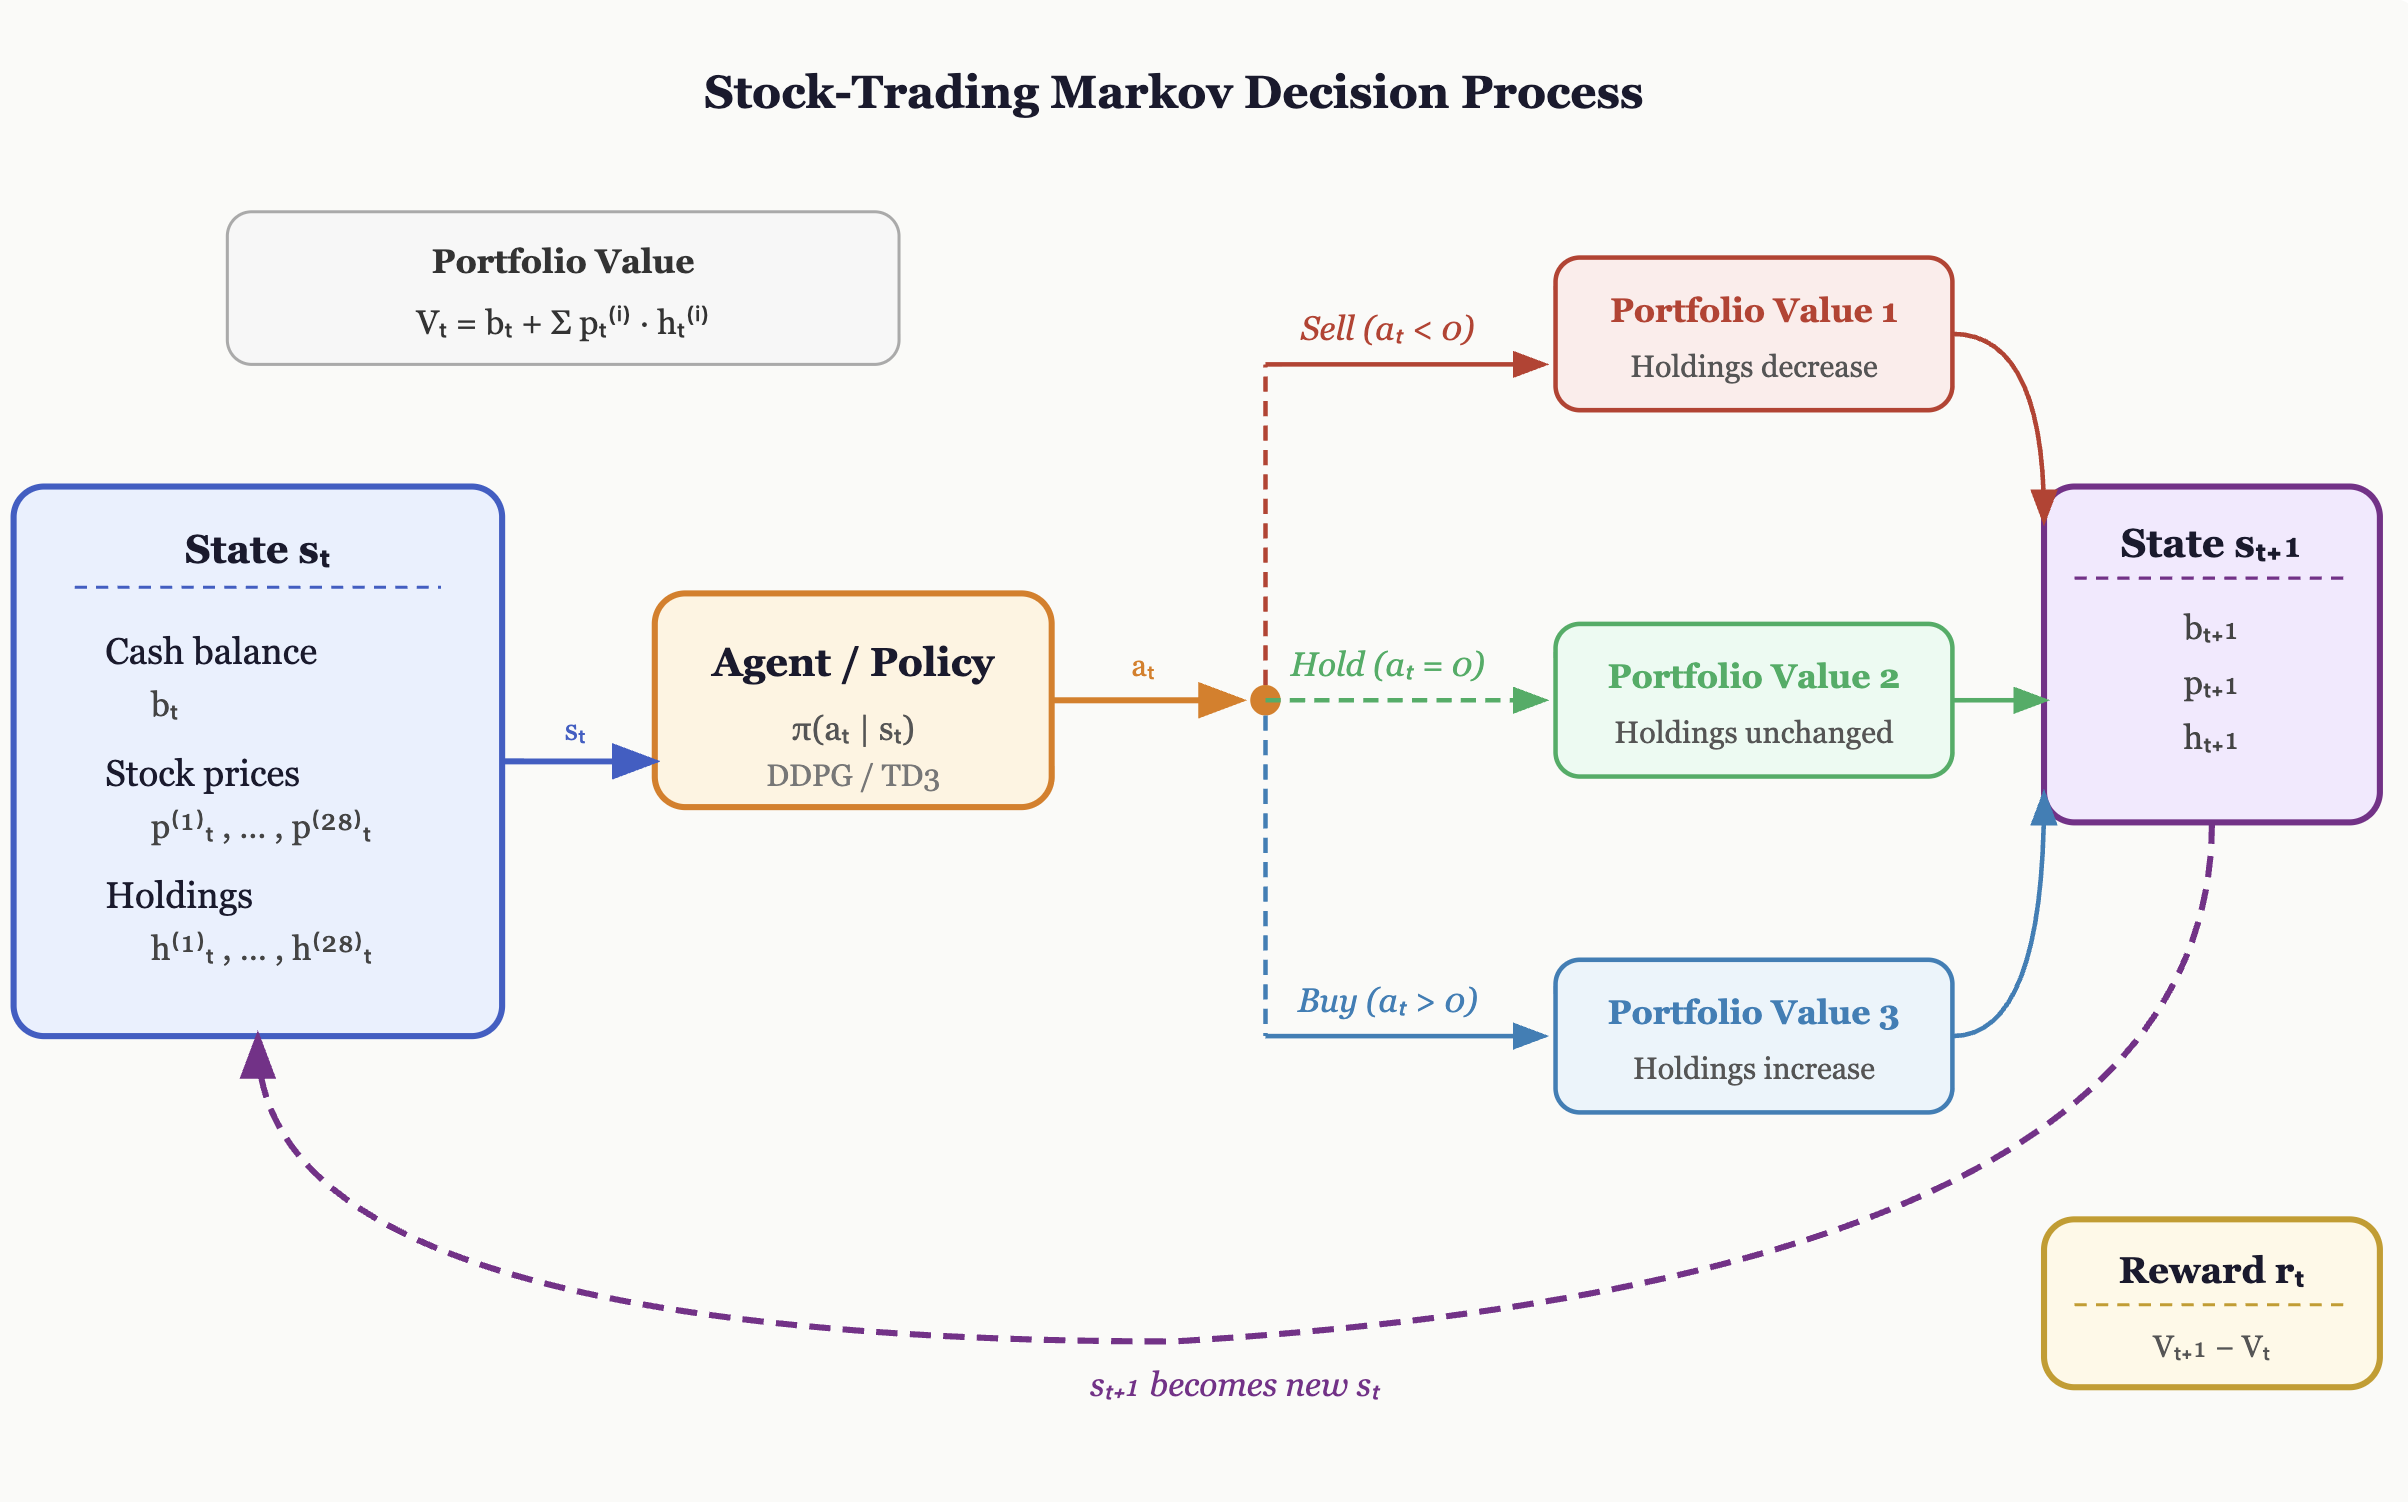
\includegraphics[width=0.95\linewidth]{resources/markov.png}
    \caption{Stock-trading MDP used in our reproduction. The agent observes cash, current prices, and current holdings, then selects bounded buy/sell actions. The environment executes trades, advances to the next trading day, and returns the change in portfolio value as the reward.}
    \label{fig:mdp_trading}
\end{figure}

The state contains cash, adjusted close prices, and holdings. Although the original paper refers to the Dow Jones 30 setting, our filtered dataset contains 28 tradable stocks, giving an observation vector of length 57:
\[
s_t =
\left[
b_t,
p_t^{(1)}, \ldots, p_t^{(28)},
h_t^{(1)}, \ldots, h_t^{(28)}
\right],
\]
where $b_t$ is cash, $p_t^{(i)}$ is the adjusted close price of stock $i$, and $h_t^{(i)}$ is the number of shares held. Each episode starts with \$10{,}000 in cash and zero holdings.

The action is a 28-dimensional trade vector,
\[
a_t =
\left[
a_t^{(1)}, \ldots, a_t^{(28)}
\right],
\]
with one action per stock. Actions are clipped, rounded, and executed as integers in
\[
a_t^{(i)} \in \{-5,-4,\ldots,0,\ldots,4,5\}.
\]
Negative values sell shares, positive values buy shares, and zero holds the position. The environment is long-only: holdings cannot become negative, and buy orders are limited by available cash. We do not model transaction costs, slippage, taxes, or borrowing.

The portfolio value is
\[
V_t = b_t + \sum_{i=1}^{28} p_t^{(i)} h_t^{(i)}.
\]
After the agent acts, the environment executes trades at the current day's prices, advances to the next trading day, and computes the reward as
\[
r_t = V_{t+1} - V_t.
\]
Thus, the agent is directly rewarded for increasing mark-to-market portfolio value. Each episode is one pass through a data split: training from 2009--2014, validation during 2015, and testing/trading from 2016--2018.


\section{DDPG}

Deep Deterministic Policy Gradient (DDPG) is an off-policy actor-critic algorithm designed for continuous action spaces \cite{lillicrap2015}. This makes it suitable for the trading environment, where the agent outputs one action value per stock before the environment converts these values into bounded buy, sell, or hold decisions. DDPG maintains two main neural networks: an actor and a critic. The actor $\mu(s|\theta^\mu)$ maps the current state $s_t$ to an action $a_t$, while the critic $Q(s,a|\theta^Q)$ estimates the expected return of taking action $a_t$ in state $s_t$.

To improve training stability, DDPG uses a replay buffer and target networks. The replay buffer stores past transitions $(s_t,a_t,r_t,s_{t+1})$, allowing the agent to train on randomly sampled mini-batches instead of highly correlated consecutive market observations. Target actor and critic networks are slowly updated versions of the main networks, and are used to compute more stable temporal-difference targets. Exploration is added by perturbing the actor's selected action with noise during training. A full DDPG training outline is included in Appendix~\ref{app:algorithms}. In this project, DDPG serves as the main reproduced algorithm because it is the method used in the original stock-trading paper \cite{liu2018practical}.

\section{TD3}

Twin Delayed Deep Deterministic Policy Gradient (TD3) is an extension of DDPG designed to reduce instability and overestimation bias in actor-critic learning \cite{fujimoto2018}. Like DDPG, TD3 uses an actor network to select continuous actions and critic networks to estimate action values. However, TD3 modifies the learning procedure in three important ways: it uses two critic networks, delays actor updates, and adds smoothing noise to target actions.

The twin critics address overestimation bias by computing the target value using the smaller estimate from two critic networks. This makes the update more conservative and reduces the chance that the actor exploits overly optimistic value estimates. TD3 also updates the actor less frequently than the critics, allowing value estimates to improve before the policy is changed. Finally, target policy smoothing adds clipped noise to the next action, making the critic less sensitive to sharp or unreliable peaks in the learned value function. A full TD3 training outline is included in Appendix~\ref{app:algorithms}. We include TD3 as a stronger comparison to DDPG in the same trading environment, especially because stock-trading rewards can be noisy and sensitive to small policy changes.

\section{Implementation}

The experiments were implemented using Stable-Baselines3 versions of DDPG and TD3, with both algorithms run through the same training and evaluation pipeline. Each model used the reproduced stock-trading environment and was trained on the original Dow Jones daily-price data, with DJIA prices provided separately for benchmark comparison.

Hyperparameters were tuned with Optuna using 10 trials per algorithm. After tuning, each algorithm was trained for 30 episodes and evaluated across three random seeds, 42, 43, and 44. The seed runs were executed in parallel, and final results were aggregated by reporting the mean and standard deviation of the agent metrics across seeds.

For consistency, DDPG and TD3 were launched with the same experimental settings: three seed workers, three Optuna jobs, and controlled CPU thread counts per job. The main difference between the two runs was the selected algorithm and the best hyperparameters found independently by Optuna.

\section{Results and Discussion}

Table~\ref{tab:trading_results} summarizes the final test-period performance of DDPG, TD3, the min-variance baseline, and DJIA. Each reinforcement learning result is reported as the mean across three random seeds, with standard deviations shown in parentheses. Both RL agents outperformed the min-variance portfolio in final portfolio value and annualized return. DDPG slightly outperformed DJIA in return, but its mean Sharpe ratio was approximately equal to DJIA, suggesting that the extra return came with slightly higher risk. TD3 produced the strongest overall result, achieving the highest final portfolio value, annualized return, and Sharpe ratio. Representative portfolio-value curves for seed 42 are included in Appendix~\ref{app:portfolio_curves}; these show the same qualitative trend, with both learned agents tracking above the min-variance baseline and TD3 ending above DDPG.

\begin{table*}[t]
\centering
\caption{Trading performance on the 2016--2018 test period. RL results are reported as mean across seeds, with standard deviation in parentheses.}
\label{tab:trading_results}
\resizebox{\textwidth}{!}{
\begin{tabular}{lcccc}
\toprule
Metric & DDPG & TD3 & Min-Variance & DJIA \\
\midrule
Initial Portfolio Value & \$10{,}000 & \$10{,}000 & \$10{,}000 & \$10{,}000 \\
Final Portfolio Value & \$16{,}141.47 $(630.95)$ & \$16{,}918.53 $(1002.53)$ & \$13{,}194.40 & \$15{,}594.84 \\
Annualized Return & 19.25\% $(1.73)$ & 21.31\% $(2.62)$ & 10.74\% & 17.76\% \\
Annualized Std. & 12.78\% $(0.99)$ & 12.67\% $(0.88)$ & 9.37\% & 11.74\% \\
Sharpe Ratio & 1.51 $(0.15)$ & 1.68 $(0.20)$ & 1.15 & 1.51 \\
\bottomrule
\end{tabular}
}
\end{table*}

The results partially reproduce the trend reported by \cite{liu2018practical}: reinforcement learning can outperform the classical min-variance baseline in this trading environment. However, our reproduced DDPG result is weaker than the original paper's reported DDPG performance. In our runs, DDPG achieved a mean final portfolio value of \$16{,}141.47, while the original paper reported \$19{,}791. This gap may be due in part to computational limitations: our models were trained for a limited number of episodes and Optuna trials, while the original paper does not fully specify the hyperparameter search process or training budget used to obtain its final result. As a result, our reproduction may not have matched the amount of tuning or training needed to reach the strongest DDPG policy.

TD3 performed better than DDPG under the same experimental setup. Its mean final portfolio value was \$16{,}918.53 compared to DDPG's \$16{,}141.47, and its mean Sharpe ratio was 1.68 compared to DDPG's 1.51. This is consistent with the design motivation behind TD3: DDPG can be sensitive to noisy or overestimated critic values, which may lead the actor toward unstable trading decisions. TD3 reduces this issue by using two critics and taking the smaller target value, delaying policy updates, and smoothing target actions \cite{fujimoto2018}. In this environment, where continuous actions are rounded into integer trades and rewards depend on noisy daily portfolio changes, these stabilizing changes likely helped TD3 produce better risk-adjusted returns.

These results suggest that future work should focus not only on more complex models, but also on more realistic and robust evaluation. Useful extensions include longer training budgets, broader hyperparameter searches, transaction costs, slippage, larger stock universes, and evaluation on additional market periods. It would also be useful to compare TD3 against other modern off-policy methods such as Soft Actor-Critic, and to test whether TD3's advantage remains under more realistic trading frictions.


\section{Conclusion}

We reproduced the stock-trading reinforcement learning setup of \cite{liu2018practical} using the same MDP formulation and historical Dow Jones data split. Our DDPG results followed the main trend of the original paper by outperforming the min-variance baseline, though they were weaker than the reported original results, likely due to a smaller training and hyperparameter-tuning budget and uncertainty around the original tuning procedure.

TD3 achieved the strongest performance in our experiments, outperforming DDPG in final portfolio value, annualized return, and Sharpe ratio. Overall, these results suggest that while DDPG can learn useful trading behavior in this environment, TD3 provides a more stable and effective alternative for this reproduced stock-trading task.

\section*{Contributions and Acknowledgements}
Both authors contributed equally to the implementation, experiments, analysis, and writing. We thank the authors of the original stock-trading DDPG repository and the developers of Stable-Baselines3 and Optuna for the tools used in this project.

% In the unusual situation where you want a paper to appear in the
% references without citing it in the main text, use \nocite
\bibliographystyle{plainnat}
\bibliography{example_paper}

%%%%%%%%%%%%%%%%%%%%%%%%%%%%%%%%%%%%%%%%%%%%%%%%%%%%%%%%%%%%%%%%%%%%%%%%%%%%%%%
%%%%%%%%%%%%%%%%%%%%%%%%%%%%%%%%%%%%%%%%%%%%%%%%%%%%%%%%%%%%%%%%%%%%%%%%%%%%%%%
% APPENDIX
%%%%%%%%%%%%%%%%%%%%%%%%%%%%%%%%%%%%%%%%%%%%%%%%%%%%%%%%%%%%%%%%%%%%%%%%%%%%%%%
%%%%%%%%%%%%%%%%%%%%%%%%%%%%%%%%%%%%%%%%%%%%%%%%%%%%%%%%%%%%%%%%%%%%%%%%%%%%%%%
\newpage
\appendix
% \onecolumn
\clearpage

\section{Algorithm Details}
\label{app:algorithms}
\FloatBarrier

\begin{algorithm}[t]
\caption{DDPG}
\label{alg:ddpg}
\begin{algorithmic}[1]
\State Initialize actor network $\mu(s|\theta^\mu)$ and critic network $Q(s,a|\theta^Q)$
\State Initialize target networks $\mu'$ and $Q'$ with the same weights
\State Initialize replay buffer $\mathcal{R}$
\For{each episode}
    \State Receive initial state $s_1$
    \For{each time step $t$}
        \State Select action $a_t = \mu(s_t|\theta^\mu) + \mathcal{N}_t$
        \State Execute action $a_t$, observe reward $r_t$ and next state $s_{t+1}$
        \State Store transition $(s_t,a_t,r_t,s_{t+1})$ in $\mathcal{R}$
        \State Sample a mini-batch of transitions from $\mathcal{R}$
        \State Compute target:
        \[
        y_i = r_i + \gamma Q'(s_{i+1}, \mu'(s_{i+1}))
        \]
        \State Update critic by minimizing:
        \[
        L = \frac{1}{N}\sum_i \left(y_i - Q(s_i,a_i)\right)^2
        \]
        \State Update actor using the policy gradient:
        \[
        \nabla_{\theta^\mu}J \approx
        \frac{1}{N}\sum_i
        \nabla_a Q(s,a)|_{s=s_i,a=\mu(s_i)}
        \nabla_{\theta^\mu}\mu(s_i)
        \]
        \State Soft-update target networks:
        \[
        \theta^{Q'} \leftarrow \tau \theta^Q + (1-\tau)\theta^{Q'},
        \qquad
        \theta^{\mu'} \leftarrow \tau \theta^\mu + (1-\tau)\theta^{\mu'}
        \]
    \EndFor
\EndFor
\end{algorithmic}
\end{algorithm}

\begin{algorithm}[H]
\caption{TD3}
\label{alg:td3}
\begin{algorithmic}[1]
\State Initialize actor network $\mu(s|\theta^\mu)$
\State Initialize two critic networks $Q_1(s,a|\theta^{Q_1})$ and $Q_2(s,a|\theta^{Q_2})$
\State Initialize target networks $\mu'$, $Q'_1$, and $Q'_2$
\State Initialize replay buffer $\mathcal{R}$
\For{each episode}
    \State Receive initial state $s_1$
    \For{each time step $t$}
        \State Select action $a_t = \mu(s_t|\theta^\mu) + \mathcal{N}_t$
        \State Execute action $a_t$, observe reward $r_t$ and next state $s_{t+1}$
        \State Store transition $(s_t,a_t,r_t,s_{t+1})$ in $\mathcal{R}$
        \State Sample a mini-batch of transitions from $\mathcal{R}$
        \State Add clipped noise to the target action:
        \[
        \tilde{a}_{i+1} = \mu'(s_{i+1}) + \epsilon,
        \qquad
        \epsilon \sim \mathrm{clip}(\mathcal{N}(0,\sigma), -c, c)
        \]
        \State Compute target using the smaller critic value:
        \[
        y_i = r_i + \gamma \min_{j=1,2} Q'_j(s_{i+1}, \tilde{a}_{i+1})
        \]
        \State Update both critics by minimizing:
        \[
        L_j = \frac{1}{N}\sum_i \left(y_i - Q_j(s_i,a_i)\right)^2,
        \qquad j \in \{1,2\}
        \]
        \If{policy update step}
            \State Update actor using $Q_1$:
            \[
            \nabla_{\theta^\mu}J \approx
            \frac{1}{N}\sum_i
            \nabla_a Q_1(s,a)|_{s=s_i,a=\mu(s_i)}
            \nabla_{\theta^\mu}\mu(s_i)
            \]
            \State Soft-update target networks
        \EndIf
    \EndFor
\EndFor
\end{algorithmic}
\end{algorithm}



%%%%%%%%%%%%%%%%%%%%%%%%%%%%%%%%%%%%%%%%%%%%%%%%%%%%%%%%%%%%%%%%%%%%%%%%%%%%%%%
%%%%%%%%%%%%%%%%%%%%%%%%%%%%%%%%%%%%%%%%%%%%%%%%%%%%%%%%%%%%%%%%%%%%%%%%%%%%%%%

\clearpage
\section{Portfolio Value Curves}
\label{app:portfolio_curves}

\begin{figure}[H]
    \centering
    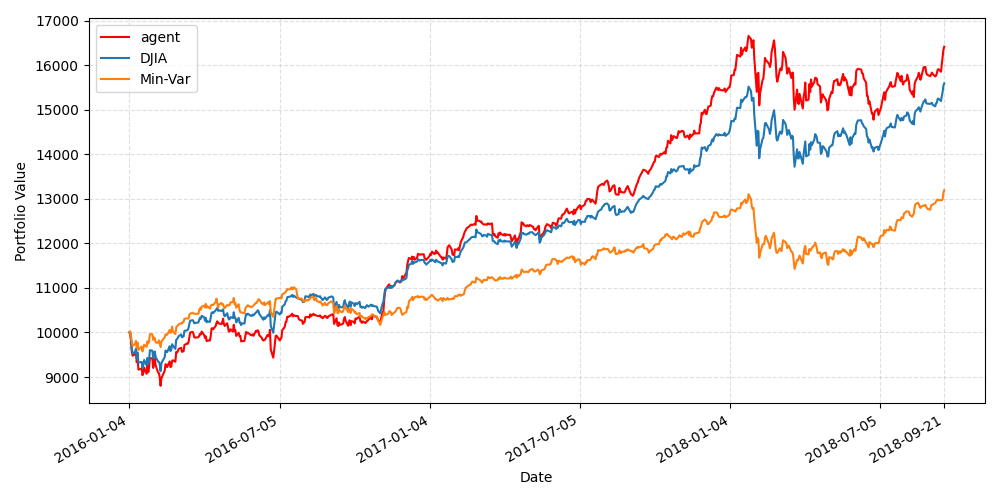
\includegraphics[width=0.95\linewidth]{resources/ddpg_model_test.png}
    \caption{DDPG portfolio value over the trading period compared against DJIA and the min-variance baseline. Representative run with seed 42.}
    \label{fig:ddpg_results}
\end{figure}

\begin{figure}[H]
    \centering
    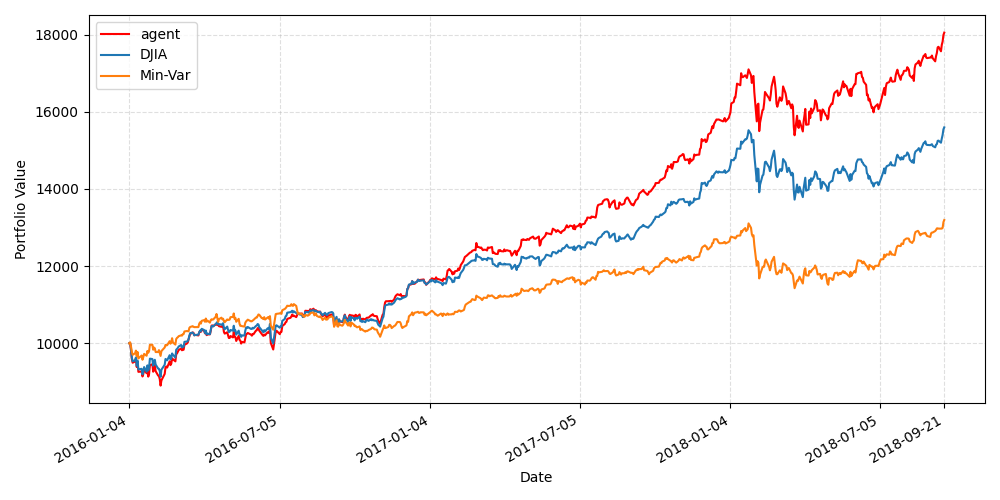
\includegraphics[width=0.95\linewidth]{resources/td3_model_test.png}
    \caption{TD3 portfolio value over the trading period compared against DJIA and the min-variance baseline. Representative run with seed 42.}
    \label{fig:td3_results}
\end{figure}

\end{document}

\newpage
\input{checklist.tex}


\end{document}